\documentclass{article}
\usepackage[utf8]{inputenc}
\usepackage{amsmath}
\newcommand{\dd}[1]{\mathrm{d}#1}
\usepackage{url}
\renewcommand{\refname}{Referencias}
\usepackage{float}
\usepackage{amssymb,enumitem}

\title{Redes Neuronales \\
  \large Trabajo Integrador \\
  }
\author{Mariano Politano }
\date{Febrero 2022}

\usepackage{natbib}
\usepackage{graphicx}
\usepackage{enumitem}

\begin{document}

\maketitle




En el presente práctico, realizamos un \textbf{autoencoder convolucional} Utilizamos el conjunto de datos MNIST.

En nuestro práctico, las imágenes tiene un tamaño de 28 x 28 píxeles en escala de grises. El dataset tiene 60000 imágenes en el conjunto de entrenamiento y 10000 imágenes en el conjunto de test.
En la Figura 1 se puede ver algunos ejemplos del dataset.
\begin{figure}[H]
\centering
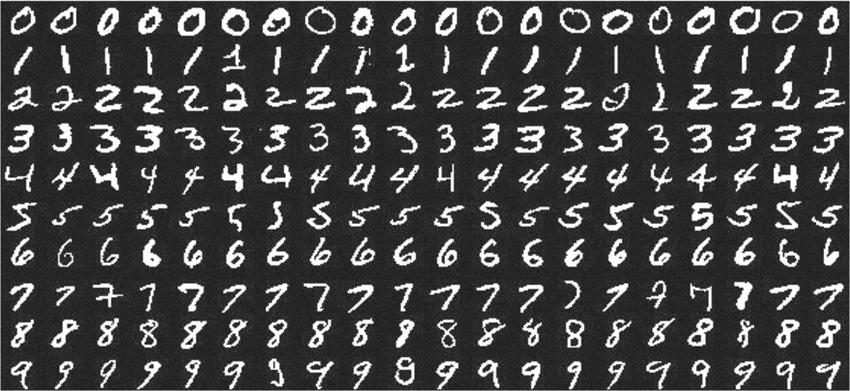
\includegraphics[width=\textwidth]{example.png}
\caption{Dataset de MNIST.}
\label{fig1}
\end{figure}

\\

Un \textbf{autoencoder} es un tipo de red neuronal no supervisada (no vemos los labels, solo nos centramos en sus características) que encuentra la función identidad a partir de compresiones que realiza a los datos de entrada de la red. Estos trabajan comprimiendo la entrada en una representación de espacio latente y luego reconstruyen la salida a partir de esta representación. Lo logra realizando el siguiente proceso: 


\begin{itemize}[noitemsep]
\item Un codificador que aprende la representación de datos en un espacio de menor dimensión, es decir, extrae las características más destacadas de los datos. Puede representarse mediante la función de codificación  h = f (x).
\item Un decodificador aprende a reconstruir los datos originales basados en la representación aprendida por el codificador. Se representa mediante la función de decodificación r = g (h)
\end{itemize}

En la siguiente figura \ref{fig2} se puede ver un diagrama de un autoencoder.

\begin{figure}[H]
\centering
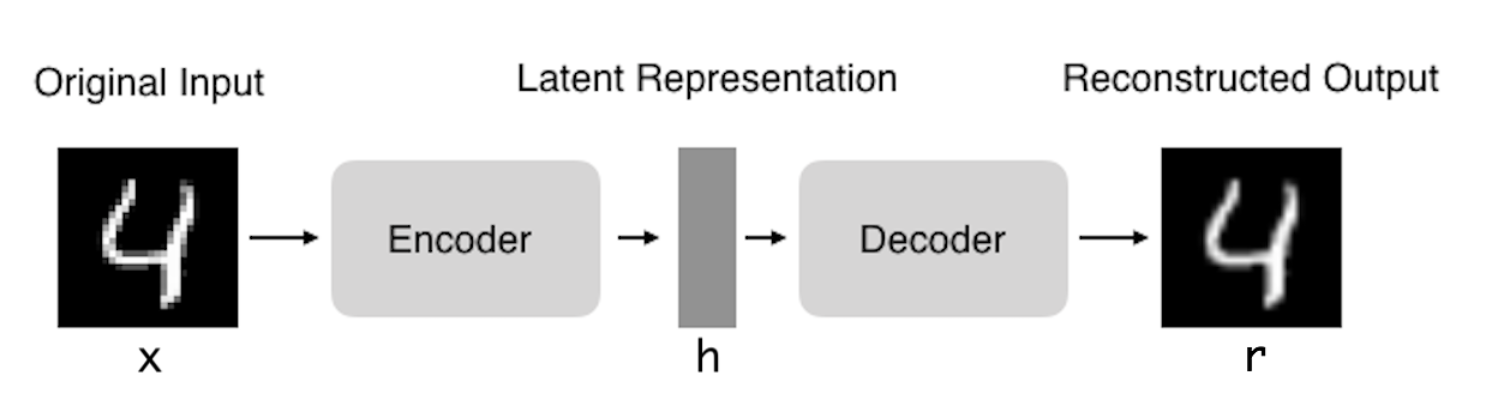
\includegraphics[width=\textwidth]{estructura.png}
\caption{Ejemplo de un autoencoder.}
\label{fig2}
\end{figure}


\section*{Resolución}

A diferencia del trabajo practico anterior, utilizamos imágenes (vectores 3D) en lugar de vectores 1D aplanados. La imagen de entrada se reduce para dar una representación latente de dimensiones más pequeñas y forzar al codificador automático a aprender una versión comprimida de las imágenes.

Para comparar los resultados con el practico anterior, utilizamos la misma función de activación Sigmoide, que limita cada probabilidad a un número en 0 y 1, y la misma función de pérdida, la función MSE, proporciona una función cuadrática de pérdida en la medida en que eleva al cuadrado y, posteriormente, promedia los varios errores; lo cual le da mucho más peso a los grandes errores (valores atípicos) que a los más pequeños.
La red se entreno durante 15 épocas. Como optimizador se utilizo Adam (Adaptive Moment Estimation) con una taza de aprendizaje de $0.001$ y minibatch de tamaño 1000.
\\

\textbf{ Caracteristica del autoencoder:} \\

Los datos de entrada se pasan a través de un codificador. Las imágenes de entrada tienen un tamaño de 28x28x1. estas imágenes se pasarán a través de capas de codificador
Tiene capas convolucionales seguidas de un max polling para reducir las dimensiones a 7x7x4
Los datos comprimidos se pasan a través de un decodificador para reconstruir los datos de entrada. En esta capa se volverá a la dimensión original 28x28x1
Utilice capas convolucionales transpuestas para aumentar el ancho y la altura de la entrada comprimida
Para evitar superposición de los kernels,iguale el tamaño del stide y del kernel. entonces usaremos stride = 2 y kernel_size = 2


\\

En la figura \ref{fig1} se puede ver que la función de pérdida a lo largo de las épocas decrece en ambas curvas, motivo por el cual se puede descartar un overfitting. Y por ende, se puede ver que a lo largo de las épocas la red mejora y tiene menos perdida, lo que significa que obtiene buenas soluciones candidatas.

\begin{figure}[H]
\centering
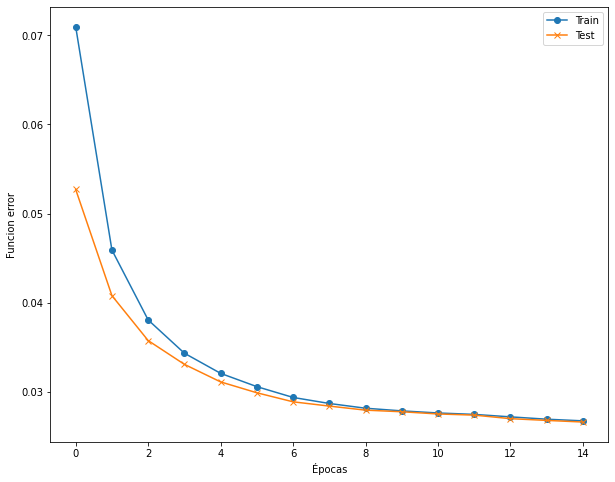
\includegraphics[width=\textwidth]{Train-vs-test.png}
\caption{Función error en train y test en base de las épocas.}
\label{fig1}
\end{figure}

En la figura \ref{fig3} se puede observar unas reconstrucciones de la entrada generada por la red.
Estas reconstrucciones, mejoran de acuerdo a cuantas capas convolucional le agregamos a esta red (Aqui se muestra para la red conformada como lo explique anteriormente). En este caso las imágenes de 28*28 se están comprimiendo a un tamaño de 7*7.

\begin{figure}[H]
\centering
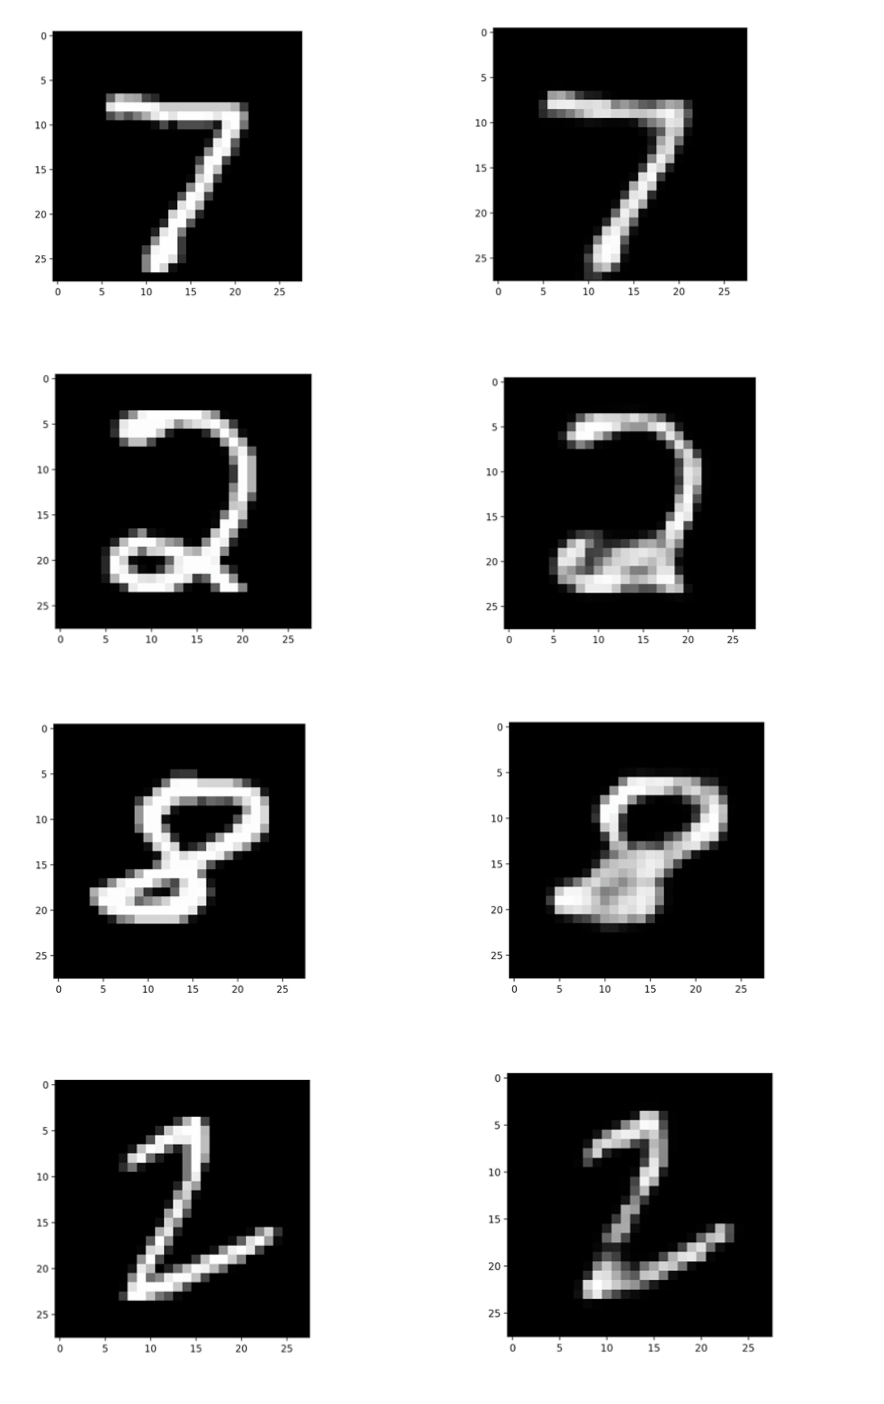
\includegraphics[width=0.7\textwidth]{reconstruccion.png}
\caption{Reconstrucciónes generada por la red. }
\label{fig3}
\end{figure}


Para concluir, realizamos una comparación de la función de perdida del practico anterior con este trabajo. Dicha comparación quedo plasmada en el gráfico  \ref{fig5}. Se puede observar que el autoencoder convolucional, rápidamente iguala a la función de perdida anterior y la supera ya en 15 épocas (cuanto mas épocas, mejor se comporta)

\begin{figure}[H]
\centering
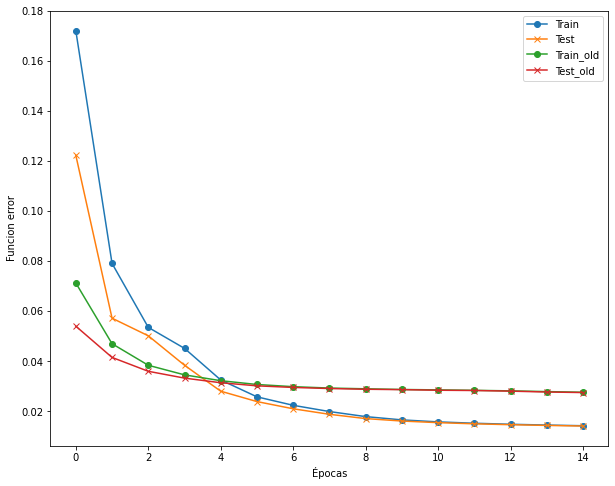
\includegraphics[width=\textwidth]{compare.png}
\caption{Función de perdida para distintos autoenconders. La referencia old, es al autoencoder realizado en el practico anterior. }
\label{fig5}
\end{figure}

\\
\


\textbf{Nota}: El práctico fue realizado en \textit{Python}, con ayuda de Gooogle Colab y se utilizo la librería Torch como se vio en clases.
    

\bibliographystyle{plain}
\bibliography{Referencias}
\begin{itemize}


\item Pizarrones de clases

\item \url{https://www.datacamp.com/community/tutorials/autoencoder-keras-tutorial#autoencoders}
\item \url{https://www.inteldig.com/2018/05/tutorial-pytorch-aprendizaje-profundo-deep-learning-en-python/}
\item \url{https://towardsdatascience.com/how-to-make-an-autoencoder-2f2d99cd5103}
\item \url{https://gist.github.com/AFAgarap/4f8a8d8edf352271fa06d85ba0361f26}
\item \url{https://medium.com/pytorch/implementing-an-autoencoder-in-pytorch-19baa22647d1}
\item \url{https://www.deeplearningitalia.com/introduzione-agli-autoencoder-2/}

\item Código del práctico:  \url{https://github.com/mpolitano/redesNueronales/ }

\end{itemize}

\end{document}